\documentclass{article}

\usepackage{latexsym}
\usepackage{bbm}
\usepackage[small,bf]{caption2}
\usepackage{graphics}
\usepackage{graphicx}
\usepackage{epsfig}
\usepackage{amsmath,amssymb,amsthm,amsfonts}
\usepackage{url}
\usepackage{hyperref}
\usepackage{enumerate}
\usepackage[most]{tcolorbox}
\usepackage{xcolor}
\usepackage{caption}
\usepackage{subcaption}

\usepackage{tikz,pgfplots}
\usetikzlibrary{shapes.geometric, arrows}

%% Page size
\setlength{\oddsidemargin}{0pt}
\setlength{\evensidemargin}{0pt}
\setlength{\textwidth}{6.5in}
\setlength{\topmargin}{0in}
\setlength{\textheight}{8.5in}

% Footnote commands.
\newcommand{\footnotenonumber}[1]{{\def\thempfn{}\footnotetext{#1}}}
\newcommand{\footnotetight}[1]{\footnote{\renewcommand\baselinestretch{1}\footnotesize #1}}

\newcommand*{\unk}{\texttt{UNK}}

\newtheorem{propo}{Proposition}[section]
\newtheorem{lemma}[propo]{Lemma}
\newtheorem{definition}[propo]{Definition}
\newtheorem{coro}[propo]{Corollary}
\newtheorem{thm}[propo]{Theorem}
\newtheorem{conj}[propo]{Conjecture}
\newtheorem{fact}[propo]{Fact}
\newtheorem{remark}[propo]{Remark}
\newtheorem{claim}[propo]{Claim}

% Create a custom environment
\newenvironment{solution}{\color{blue}}{}

\setlength{\parindent}{0pt}

\begin{document}
\section{Understanding Attentions}
\subsection{Background on Self-Attention}
\begin{solution}
  No submission required in this section.
\end{solution}

\subsection{Selection via Attention}
\begin{enumerate}
  \item Define a \textit{query} vector $q$ ($\in \mathbb{R}^3$) to ``select'' (i.e., return) the first \textit{value} vector $v_0$. Briefly explain how you get your solution.
  
  \begin{solution}
    To ``select'' the first \textit{value} vector, we want to have an attention after 
    the softmax to be a vector $\begin{bmatrix}
      1 & 0 & 0 & 0
    \end{bmatrix} \in \mathbb{R}^{1 \times 4}$. Since softmax takes the exponential of all the entries in the pre-softmax attention $A$ and weight them accordingly, we basically want to form $A$ to be some entries s.t. \textbf{taking exponentials of the first entry would be much greater than the others so that the denominators of the others don't matter that much.} The easiest way to define the smaller ones to be overriden by the first entry is just use 0 because $\exp(0) = 1$. Now we have control that all the entries except the first one in $A'$ (which denotes the attention after the softmax layer) to be 1. We can design a large exponents $k$ s.t. $\frac{\exp(k)}{\exp(k) + 1 + 1 + 1} \rightarrow 1$. An easy choice could just be $k=100$, which is definitely an overkill but good enough. Since we know $A = q K^T$, we simply use \texttt{torch.linalg.lstsq} to find out the corresponding $q$ with $K$ and $A$ given. The resulting $q = \begin{bmatrix}
      44.6093 & 28.4705 & 31.0986
    \end{bmatrix}$. A note on approximating $q$ using \texttt{lstsq} is that the resulting $q$ might not completely satisfy the equation we give because it's only an approximation as $K$ is not invertible. Therefore, there could be differences between the desired $A$ and the approximated $\hat{A} = \hat{q} K^T$.
  \end{solution}

  \item Define a \textit{query} matrix $Q$ ($\in \mathbb{R}^{4 \times 3}$) which results in an identity mapping -- select all the \textit{value} vectors. Briefly explain how you get your solution.
  
  \begin{solution}
    With the similar intuition from previous part, this time we want to design a matrix $Q \in \mathbb{R}^{4 \times 3}$ where each individual query $q_i \in \mathbb{R}^{1 \times 3}$ should result in an attention $A_i'$ after softmax to be close to $\begin{bmatrix}
      a'_0, a'_1, a'_2, a'_3
    \end{bmatrix}$ where $a'_i = 1$. The full attention matrix $A'$ following this would just be an identity matrix $I_4 \in \mathbb{R}^{4 \times 4}$. Since each query doesn't affect the others, we can design each row of $A$ the same way as previous section. Hence,
    $A = \begin{bmatrix}
      k & 0 & 0 & 0
      \\ 0 & k & 0 & 0
      \\ 0 & 0 & k & 0
      \\ 0 & 0 & 0 & k
    \end{bmatrix}$ where $k = 100$ can be a choice large enough for ``selection''. Then we use the same function to approximate $Q$ with given $K$ and $A$. The resulting $Q = \begin{bmatrix}
      44.6093 &  28.4705 &  31.0986 \\
      74.2993 &  24.4711 & -43.9832 \\
      9.9978 & -24.5389 & -51.8660 \\ 
      73.9117 & -69.2530 & 27.8533
    \end{bmatrix}$. The same approximation note on \texttt{lstsq} from above also applies here.
  \end{solution}


  \item What does attention's ability to copy / select from input tokens when creating outputs imply for language modeling? In other words, why might this be desirable? (1-3 sentences)
  
  \begin{solution}
    If the goal is to model the natural language, the ability to ``select'' from input tokens when creating outputs allows the model to focus on some certain section of the previous sentence that largely affects the next token. For instance, a sentence like "I feel sick today, so I have to do my homework [output]." The output should focus on "sick" and "today" more than "have" in order to produce reasonable output. Selecting ability is closer to how people treat natural language and can also be justified by looking at the semantic parsing tree in linguistic.
  \end{solution}

\end{enumerate}

\subsection{Averaging via Attention}
  \begin{enumerate}
    \item Define a \textit{query} vector $q$ ($\in \mathbb{R}^{3}$) which averages all the \textit{value} vectors. Briefly explain how you get your solution.
    
    \begin{solution}
      In order to find the query that average all the vectors, the attention $A'$ after the softmax should be close to $\begin{bmatrix}
        \frac{1}{4} & \frac{1}{4} & \frac{1}{4} & \frac{1}{4}
      \end{bmatrix}$. Considering softmax weighting after taking the exponentials, having $A$ with all zeros is actually a good choice because $\exp(0) = 1$ and the softmax would just make each entry $\frac{\exp(0)}{\exp(0) + \exp(0) + \exp(0) + \exp(0)} = \frac{1}{4}$. To get such $A$ with all zeros, having $q$ to be all zeros is sufficient. i.e. $q = \begin{bmatrix}
        0 & 0 & 0
      \end{bmatrix}$.
    \end{solution}


    \item Define a \textit{query} vector $q$ ($\in \mathbb{R}^{3}$) which averages the first two \textit{value} vectors. Briefly explain how you get your solution.
    
    \begin{solution}
      To average over only the two values, it mixes the concepts from the previous subsection and this section. Essentially, we want to design the $A$ s.t. after the softmax $A'$ would have the first two entries to be closer to each other in order to obtain an averaging effect. In addition, we also need to ensure that the third and fourth entries in the same attention should be much smaller (negligible) s.t. it won't affect too much on ``selecting'' and ``averaging'' the first two entries. Concretely, we hope $A' = \begin{bmatrix}
        a'_0 & a'_1 & a'_2 & a'_3
      \end{bmatrix}$ s.t. $a'_0 \approx a'_1$ (averaging) and $a'_0, a'_1 \gg a'_2, a'_3$ (selecting and ignoring last two values). 

      As mentioned in previous section, there exists an approximation challenge in that even if we design an $A$, there is no guarantee such $Q$ exists to satisfy $QK^T = A$. Therefore, in this problem, we carefully design the constants in $A$ in order to find a good approximate (feasible) $Q$. Instead of going crazy like $k = 100$ for overriding terms, we use $k=3$. i.e. $A = \begin{bmatrix}
        3 & 3 & a_2 & a_3
      \end{bmatrix}$. Now the remaining challenge is to design the $a_2, a_3$ s.t. $e^{a_2}, e^{a_3} \ll e^{3}$. Then we consider the feasibility of $A = q K^T$. $q$ is essentially the weights to construct a linear combination of the three columns in $K$ to form $A$.Considering \texttt{K[2]} and \texttt{K[3]} both have negative terms and $\exp(c)$ is also small when $c$ is negative, we can let $a_2$ and $a_3$ to be some negative numbers. Moreover, to further improve feasibility of $q$, we see \texttt{K[0]} and \texttt{K[1]} both have large terms in their first column, so the weight for the linear combination of columns should be higher to construct larger \texttt{A[0], A[1]}. However, we see that \texttt{K[3]} actually has high value for the first column as well. If the weight for this column is high in order to satisfy higher first two rows, the resulting \texttt{A[3]} would probably also be higher than \texttt{A[2]}. Therefore, instead of choosing the same negative numbers for $a_2$ and $a_3$, I choose $a_2 = -2$ and $a_3 = -3$ because $a_2$ is more likely to be less negative considering the first column to get feasibility. This wouldn't matter in terms of the property of attention we care about because $\exp(-2)$ and $\exp(-3)$ are both a lot less than $\exp(3)$.
    \end{solution}

    \item What does the ability to average / aggregate (in some cases selectively) imply for language modeling? In other words, why might this be desirable? (1-3 sentences)
    
    \begin{solution}
      With the selection ability, a model can focus on certain words that contribute to the probability of the next word. However, the information flow between words that form context is much more than selecting certain words to focus on. Instead, the ability to aggregate information from different words to imply the next token is essential in natural language. This ability is somewhat shown in our section 1.3. It would help with understanding the interaction between tokens better than simply picking individual words.
    \end{solution}
\end{enumerate}

\subsection{Interactions within Attention}
\begin{enumerate}
    \item Come up with a replacement for only the third \textit{key} vector $k_2$ such that the result of attention with the same unchanged \textit{query} $q$ from \S 1.3.2 averages the first three \textit{value} vectors. Briefly explain how you get your solution.
    
    \begin{solution}
      We already know $k_0$ and $k_1$ are keys that result in large weights in $A'$ after softmax with our $q$ because we design the $q$ accordingly. Now, as long as we make the third entry in $A$ to be roughly the same as $a_0$ and $a_1$, then we are set. And what does our designed query $q$ tell us is that $k_0$ and $k_1$ are good keys to get large enough weights to disregard $k_3$'s resulting weights. So choosing $k_2 = k_0$ or $k_2 = k_1$ can result in $a_2 \approx a_0, a_1$ and $a_2 \gg a_3$. In the code, we simply choose $k_2 = k_0$.
    \end{solution}

    \item Come up with a replacement for only the third \textit{key} vector $k_2$ such that the result of attention with the same unchanged \textit{query} $q$ from \S 1.3.2 returns the third \textit{value} vector $v_2$.
    However, there is the condition that $k_2$ should have length $=1$. This is not usually a restriction in attention, but is only for this problem. Briefly explain how you get your solution.

    \item Why is altering $k_2$ able to impact an output which previously only considered the first two tokens? (2-4 sentences)
    
    \begin{solution}
      The intuition behind query-key-value is that when query is to retrieve (pay attention) to values with desired keys that the query is designed to. Hence, we can modify the key if we know how the query is designed to ``draw attention'' to the value we are interested in.
    \end{solution}
\end{enumerate}

\newpage

\section{Building Your Own Mini Transformer}
\subsection{Implementing Attention from Scratch}
\begin{solution}
  Code submitted through gradescope
\end{solution}

\subsection{Experiment with Your Implementation of Attention}
\subsubsection{Baseline}
\begin{solution}
  \begin{table}[!htbp]
    \caption{Baseline}
    \label{baseline}
    \begin{center}
      \begin{tabular}{| c | c | c | c | c | c |}
        \hline
        & Train & Dev & Normal Sample & Weird Sample & Long Sample \\ \hline
        Perplexity & 401.04 & 380.80 & 280.21 & 12820.43 & 428.35 \\ \hline
        Loss & 5.73 & 5.69 & 5.63 & 9.45 & 6.05 \\ \hline
      \end{tabular}
    \end{center}
  \end{table}

  \begin{enumerate}
    \item \textbf{Setup}: The baseline is set up as the given starter code where we use \texttt{gpt-nano} configuration with block size of 1024. The normal sample is the provided sentence for loss and perplexity calculation demo: \textit{Thank you so much Liwei and Taylor for all your help with this !}. The weird sample is the provided sample in demo: \textit{After learning language models model natural language}. The long sample is found online: \textit{On offering to help the blind man, the man who then stole his car, had not, at that precise moment, had any evil intention, quite the contrary, what he did was nothing more than obey those feelings of generosity and altruism which, as everyone knows, are the two best traits of human nature and to be found in much more hardened criminals than this one, a simple car-thief without any hope of advancing in his profession, exploited by the real owners of this enterprise, for it is they who take advantage of the needs of the poor.}
  \end{enumerate}

\end{solution}

\subsubsection{Sine-Cosine Positional Encoding}

\begin{solution}
  \begin{table}[!htbp]
    \caption{Sine-Cosine Positional Encoding}
    \label{sinusoidal}
    \begin{center}
      \begin{tabular}{| c | c | c | c | c | c |}
        \hline
        & Train & Dev & Normal Sample & Weird Sample & Long Sample \\ \hline
        Perplexity & 525.31 & 485.56 & 437.24 & 10368.04 & 505.39 \\ \hline
        Loss & 6.03 & 5.96 & 6.08 & 9.24 & 6.22 \\ \hline
      \end{tabular}
    \end{center}
  \end{table}

  \begin{enumerate}
    \item \textbf{Motivation}
    
    The model originally used learned embeddings for positional encoding. Since most of the sequences are not at maximum sequence length, the encoding might not be learned well for longer sequences. We implemented sinusoidal positional encoding and examine its performance.
    \item \textbf{Setup}
    
    The setup is the same as the baseline. The only difference is the positional encoding. It's using sinusoidal positional encoding specified as 
    $$PE_{k, i} = \begin{cases}
       \sin (\frac{k}{10000^{i / d}}) &i = 2 * m
      \\ \cos (\frac{k}{10000^{i / d}}) &i = 2 * m + 1
    \end{cases}$$
    where $k$ is the position of the token and $i$ is the $i$th dimension in the embedding.

    \item \textbf{Analysis}
    
    Comparing table 1 and table 2, we see that sinusoidal positional encoding actually hurts the performance in general. This makes sense in that the distribution of the training text has densely distributed sentences with similar length. Therefore, the learned positional encodings are generally better in those lengths. In addition, in training and evaluation set, those lengths appear more often. However, when we compare the long sample, we find that even sinusoidal positional encoding hurts the performance. This is counter-intuitive but we hypothesize that the sample size is not enough. There needs more long sequence samples for this set of evaluation.
  \end{enumerate}
\end{solution}

\subsubsection{Fusion Multi-head Attention}
\begin{solution}
  \begin{table}[!htbp]
    \caption{Shuffle Multi-head Attention}
    \begin{center}
      \begin{tabular}{| c | c | c | c | c | c |}
        \hline
        & Train & Dev & Normal Sample & Weird Sample & Long Sample \\ \hline
        Perplexity & 404.63 & 383.59 & 322.56 & 13879.92 & 419.71  \\ \hline
        Loss & 5.74 & 5.70 & 5.77 & 9.53 & 6.03  \\ \hline
      \end{tabular}
    \end{center}
  \end{table}

  \begin{table}[!htbp]
  \caption{Shift-by-one Multi-head Attention}
  \begin{center}
    \begin{tabular}{| c | c | c | c | c | c |}
      \hline
      & Train & Dev & Normal Sample & Weird Sample & Long Sample \\ \hline
      Perplexity & 402.10 & 382.20 & 299.93 & 14801.54 & 425.183 \\ \hline
      Loss & 5.73 & 5.69 & 5.70 & 9.60 & 6.05  \\ \hline
    \end{tabular}
  \end{center}
  \end{table}

  \begin{table}[!htbp]
  \caption{Re-weight Multi-head Attention}
  \begin{center}
    \begin{tabular}{| c | c | c | c | c | c |}
      \hline
      & Train & Dev & Normal Sample & Weird Sample & Long Sample \\ \hline
      Perplexity & 362.84 & 345.57 & 2178713.25 & 2550125904.81 & 341466.20 \\ \hline
      Loss & 5.63 & 5.59 & 14.59 & 21.65 & 12.74 \\ \hline
    \end{tabular}
  \end{center}
  \end{table}
  
  \begin{enumerate}
    \item \textbf{Motivation}
    
    Multi-head attention is used to have multiple projection matrices for query-key-value that describes different subspaces that total up to $d$ dimensions. Then we concatenate those attentions in each subspace together after computing the output value in each subspace. With this approach, a question to ask could be what exactly different parts of subspace in embeddings do? Are they correlated? We can try to answer this question by shuffling the output value in each head before concatenating them back together. Hypothetically, if each head doesn't work like an expert, then this shuffling shouldn't affect too much. Another question to ask is what would happen if we shift the head's subspace by one. Hypothetically, this should not affect too much in that each layer's heads are still getting the same piece of subspace because the shifting happens deterministically. This shifting should be invariant from the performance. Finally, we try to see if one head can be more important than the others and whether re-weighting the values could be helpful.

    \item \textbf{Setup}
    
    We use the same 3 head setting as the baseline. There are three variants to deal with merging heads.
    \begin{enumerate}
      \item \textbf{Shuffling}: Unlike traditional concatenation, we concatenate them in random orders. e.g. Traditional merging heads looks like $\begin{bmatrix}
        O^{(1)} & O^{(2)} & ... & O^{(h)}
      \end{bmatrix}$. The shuffling merging heads looks like $\begin{bmatrix}
        O^{(s_1)} & O^{(s_2)} & ... & O^{(s_h)}
      \end{bmatrix}$ where $\{ s_1, ..., s_h \}$ is random permutation of 1 to $h$. This shuffling happens for each layer.
      \item \textbf{Shift by one}: In this setting we concatenate the output by $\begin{bmatrix}
        O^{(2)} & O^{(3)} & ... & O^{(h)} & O^{(1)}
      \end{bmatrix}$ for each layer. This happens for each layer.
      \item \textbf{Re-weight output}: In this setting we re-weight the output value from each head by their matrix norm. The higher the matrix norm is, the more weight they gain as a result. The ordering of concatenation stays the same.
    \end{enumerate}
    
    \item \textbf{Analysis}
    
    To better analyze the effects, we form another perplexity table for comparison.

    \begin{table}[!htbp]
      \caption{Perplexity}
      \begin{center}
        \begin{tabular}{| c | c | c | c | c | c |}
          \hline
          & Train & Dev & Normal Sample & Weird Sample & Long Sample \\ \hline
          Baseline & 401.04 & 380.80 & \textbf{280.21} & \textbf{12820.43} & 428.35 \\ \hline
          Shuffle & 404.63 & 383.59 & 322.56 & 13879.92 & \textbf{419.71}  \\ \hline
          Shift-by-one & 402.10 & 382.20 & 299.93 & 14801.54 & 425.183 \\ \hline
          Re-weight & \textbf{362.84} & \textbf{345.57} & 2178713.25 & 2550125904.81 & 341466.20 \\ \hline
        \end{tabular}
      \end{center}
    \end{table}

    \begin{solution}
      \begin{enumerate}[(a)]
        \item It turns out neither shuffle nor shift-by-one has huge effects on the perplexity. This implies that there is no explicit expertise in the subspace of output to some extent.
        \item For re-weighting, it turns out to perform really well on both training and dev set. Weighting more on heads actually helps. However, when it comes to single samples, the perplexity blows up really high. This behavior is not investigated into further for the sake of the length of this problem. One possibility is that the weighting mechanism can completely ruin the model's ability to generalize. One way to possibly work around is turn off the re-weighting in inference time.
      \end{enumerate}
    \end{solution}

  \end{enumerate}
\end{solution}

\newpage

\section{HuggingFace}
\begin{itemize}
  \item[\textit{Step 1:}] \textit{Defining PyTorch Dataset and Dataloader}
  
  \begin{itemize}
    \item[\textbf{Q1.1:}] Explain the usages of the following arguments when you encode the input texts: \texttt{padding}, \texttt{max\_length}, \texttt{truncation}, \texttt{return\_tensors}.
    
    \begin{solution}
      \texttt{padding} is used as a flag for tokenizer to determine whether to append padding tokens at the end of the sentence if the sentence doesn't have \texttt{max\_length}. \texttt{max\_length} defines the maximum sequence length we want each sample to have. \texttt{truncation} is used as a flag for tokenizer to determine whether to trim tokens after the \texttt{max\_length} s.t. each sentence has at most \texttt{max\_length} tokens. \texttt{return\_tensors} is just the type of tensors we want. Since we are using \texttt{PyTorch} framework, we pass in \texttt{pt}.
    \end{solution}

    \item[\textbf{Q1.2:}] For the above arguments, explain what are the potential advantages of setting them to the default values we provide.
    
    \begin{solution}
      Having both \texttt{padding} and \texttt{truncation} is nice because there would be exactly \texttt{max\_len} tokens for each sample. The \texttt{max\_len} is set to be 512 which is a reasonable number. \texttt{return\_tensors} is set to be \texttt{pt} for we are using \texttt{PyTorch}.
    \end{solution}
  \end{itemize}
  
  \item[\textit{Step 2:}] \textit{Loading Data}
  
  \begin{itemize}
    \item[\textbf{Q2.1:}] What are the lengths of train, validation, test datasets?
    
    \begin{solution}
      Length of train dataset: 6920
      
      Length of validation dataset: 872
      
      Length of test dataset: 1821
    \end{solution}
    
    \item[\textbf{Q2.2:}] Explain the role of each of the following parameters: \texttt{batch\_size}, 
    \texttt{shuffle}, \texttt{collate\_fn}, \texttt{num\_workers} given to the \texttt{DataLoader} in the above code block.

    \begin{solution}
      \texttt{batch\_size}: This is used as the number of samples to load at once. We need to load data batch by batch because loading a full dataset is usually not feasible considering the memory of GPU.

      \texttt{shuffle}: This is used to decide whether to shuffle the ordering of dataset in the dataloader. If \texttt{shuffle=True}, iterating through the dataloader would have samples in random order.

      \texttt{collate\_fn}: This is the function applied for every batch upon it's loaded. In our case, tokenization is applied for every batch of text and label.

      \texttt{num\_workers}: This is used to decide number of workers on CPU to load data in parallel. This can be used to take advantage of multi-processing for faster loading.
    \end{solution}
    
    \item[\textbf{Q2.3:}] Write the \textbf{type} and \textbf{shape} (if the type is tensor) of \texttt{input\_ids}, \texttt{attention\_mask}, and \texttt{label\_encoding} in \texttt{batch} and explain \textbf{what these elements represent}.
    
    \begin{solution}
      \texttt{input\_ids}: The type of it is \texttt{torch.Tensor} with shape \texttt{(B, 45)} where \texttt{B} is the batch size, which is 64 when dataloader is initialized. The 45 is specific to this dataset which can be the maximum sequence length. Each tensor in this batch represents the input sequence in tokens indexed by the tokenizer. Each id is a token in the vocabulary of tokenizer.

      \texttt{attention\_mask}: The type of it is \texttt{torch.Tensor} with shape \texttt{(B, 45)} where \texttt{B} is the batch size, which is 64 when dataloader is initialized. Each tensor in this batch contains 1 for all valid tokens and 0 for all paddings to avoid paying attentions to padding tokens appended at the end of the sentence up to max sequence length.

      \texttt{label\_encoding}: The type of it is \texttt{torch.Tensor} with shape \texttt{(B,)} where \texttt{B} is the batch size, which is 64 when dataloader is initialized. Each tensor in this batch represents the label of each sample in the batch. In this case, we have binary labeling so it's either 0 or 1.
    \end{solution}
  \end{itemize}
  
  \item[\textit{Step 3:}] \textit{Training and Evaluation}

  \begin{itemize}
    \item[\textbf{Q3.1:}] For the three lines of code you implemented for computing gradients and updating parameters using optimizer, explain what each of the lines does, respectively.
    
    \begin{solution}
      \texttt{optimizer.zero\_grad()}: In \texttt{PyTorch}, gradients can get accumulated if backward propagation is called multiple times. This line zeros out the existing gradients in the computation graph in order to prepare for the next backward propagation independent from the previous one.
      
      \texttt{loss.backward()}: This calculates all gradients of the tensors in the computation graph obtained during forward pass and set all the gradients in each tensor's \texttt{grad} field.
      
      \texttt{optimizer.step()}: The optimizer takes an update step using all tensors' \texttt{grad} set by the backward call previously. Note that this only applies to tensors included in the optimizer's parameter group.
    \end{solution}
    
    \item[\textbf{Q3.2:}] Explain what setting the model to training and evaluation modes do, respectively.

    \begin{solution}
      In training mode, layers like dropout and batch normalization would stay activated and used. On the other hand, in eval mode, the model's dropout layer and batch normalization would be disabled for inference purpose.
    \end{solution}
    
    \item[\textbf{Q3.3:}] Explain what \texttt{with torch.no\_grad()} does in the \texttt{evaluation()} function.

    \begin{solution}
      \texttt{with torch.no\_grad()} disables all gradient calculation globally. This includes all kinds of tensors including input, loss, and model parameters. The reason why we have this in evaluation is to save memory because there is no need to calculate gradients in inference time.
    \end{solution}
  \end{itemize}

  
  \item[\textit{Step 4:}] \textit{Main Training Loop}

  \begin{itemize}
    \item[\textbf{Q4.1:}] With the following default hyperparameters we provide, plot both training and validation loss curves across 10 epochs in a single plot ($x$-axis: num of the epoch; $y$-axis: acc). You can draw this plot with a Python script or other visualization tools like Google Sheets. (\texttt{batch\_size} = 64, \texttt{learning\_rate} = 5e-5, \texttt{num\_epochs} = 20, \texttt{model\_name} = "roberta-base")
    
    \begin{figure}[!htbp]
      \centering
      \begin{subcaptiongroup}
        \centering
        \parbox[b]{.4\textwidth}{%
        \centering
        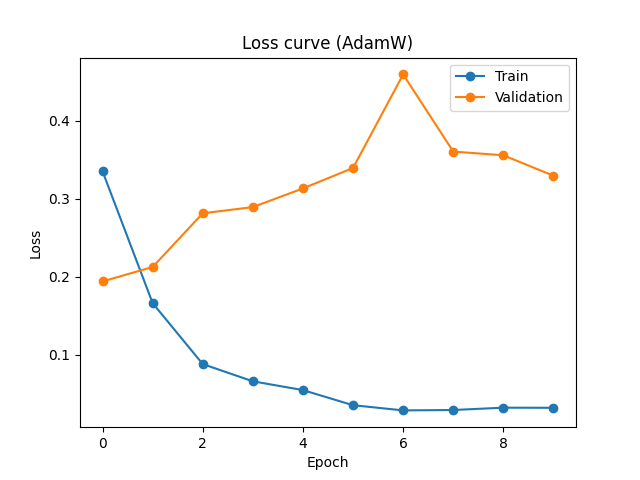
\includegraphics[width=0.4\textwidth]{loss_curve_epoch_10_AdamW.png}
        \caption{AdamW loss curve}\label{AdamW-loss-4.1}}%
        \centering
        \parbox[b]{.4\textwidth}{
        \centering
        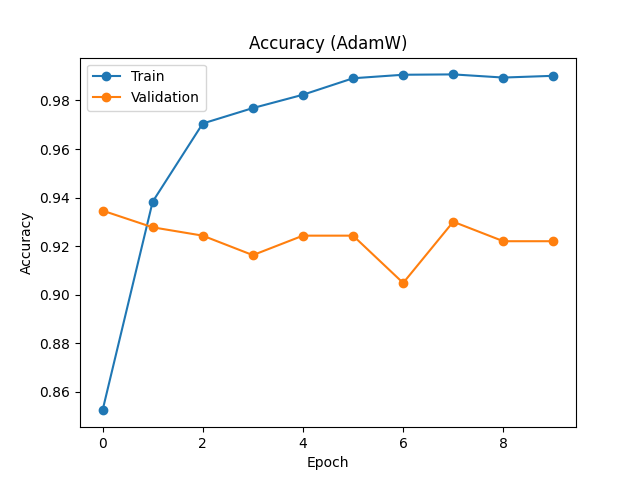
\includegraphics[width=0.4\textwidth]{acc_curve_epoch_10_AdamW.png}
        \caption{AdamW acc curve}\label{AdamW-acc-4.1}}
      \end{subcaptiongroup}
    \end{figure}
    
    \item[\textbf{Q4.2:}] Describe the behaviors of the training and validation loss curves you plotted above. At which epoch does the model achieve the best accuracy on the training dataset? What about the validation dataset? Do training and validation curves have the same trend? Why does the current trend happen?
    
    \begin{solution}
      The model achieves the best training accuracy at the 8th epoch (The plot is zero-indexed). The model achieves the best validation accuracy at the first epoch. The validation curve has decreasing trend while the training has increase trend. This is likely coming from overfitting. The reason why overfitting starts at the beginning here is that we load a pretrained model which is already performative and generalize well.
    \end{solution}
    
    \item[\textbf{Q4.3:}] Why do you shuffle the training data but not the validation data?
    
    \begin{solution}
      In stochastic gradient descent and the momentum variants like AdamW, Adam, and others, randomly sampling a batch is the ideal behavior. However, to take advantage of full data, we shuffle the order and iterating over the batches as an alternative of sampling batches. If we don't shuffle the data during training, it's likely that the model is memorizing the patterns of each batch and can perfectly minimize those batch losses very well without generalization. In validation, we don't need this sampling because we only care about evaluation.
    \end{solution}
    
    \item[\textbf{Q4.4:}] Explain the functionality of optimizers.
    
    \begin{solution}
      Optimizer is the implementation of optimization techniques and serves as an interface for us to develop with. Essentially, it takes the parameters we care about. e.g. the model's trainable parameters. Then, when calling \texttt{optimizer.step()}, we ask the optimizer to do an update step based on the gradients that each parameter currently holds and the algorithm initialized like Adam, SGD, and so on.
    \end{solution}
    
    \item[\textbf{Q4.5:}] Experiment with two other optimizers defined in \texttt{torch.optim} for the training the model with the default hyperparameters we give you. What is the difference between \texttt{AdamW} and these two new optimizers? Back up your claims with empirical evidence.
    
    \begin{figure}[!htbp]
      \centering
      \begin{subcaptiongroup}
        \centering
        \parbox[b]{.3\textwidth}{%
        \centering
        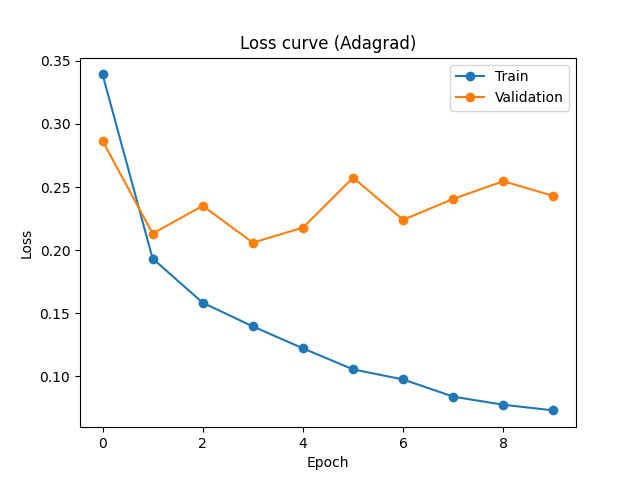
\includegraphics[width=0.3\textwidth]{loss_curve_epoch_10_Adagrad.png}
        \caption{Adagrad loss curve}\label{Adagrad-loss}}%
        \parbox[b]{.3\textwidth}{%
        \centering
        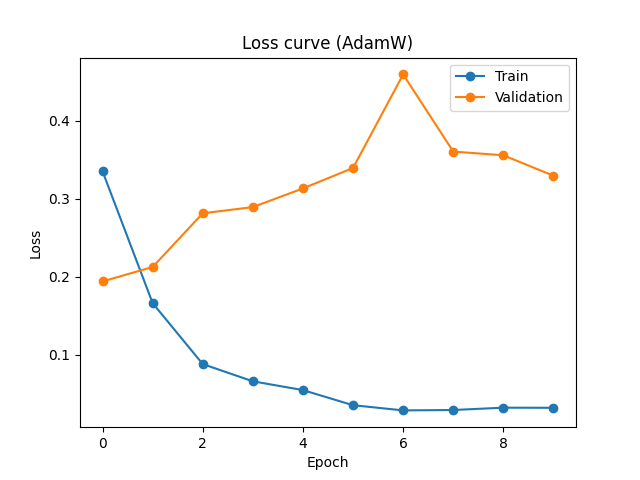
\includegraphics[width=0.3\textwidth]{loss_curve_epoch_10_AdamW.png}
        \caption{AdamW loss curve}\label{AdamW-loss}}%
        \centering
        \parbox[b]{.3\textwidth}{
        \centering
        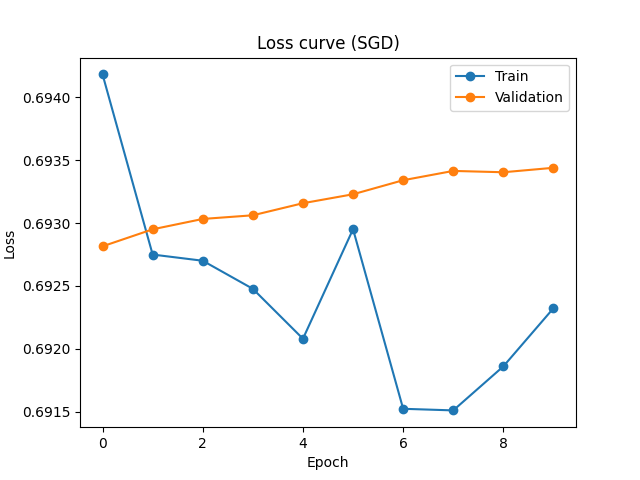
\includegraphics[width=0.3\textwidth]{loss_curve_epoch_10_SGD.png}
        \caption{SGD loss curve}\label{SGD-loss}}
      \end{subcaptiongroup}
    \end{figure}

    \begin{figure}[!htbp]
      \centering
      \begin{subcaptiongroup}
        \centering
        \parbox[b]{.3\textwidth}{%
        \centering
        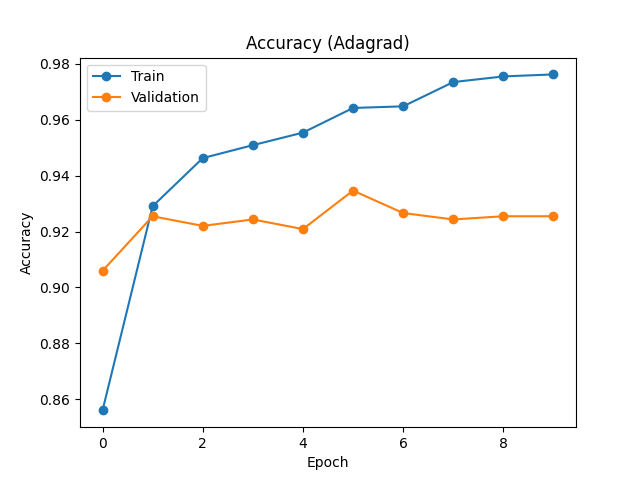
\includegraphics[width=0.3\textwidth]{acc_curve_epoch_10_Adagrad.png}
        \caption{Adagrad acc curve}\label{Adagrad-acc}}%
        \parbox[b]{.3\textwidth}{%
        \centering
        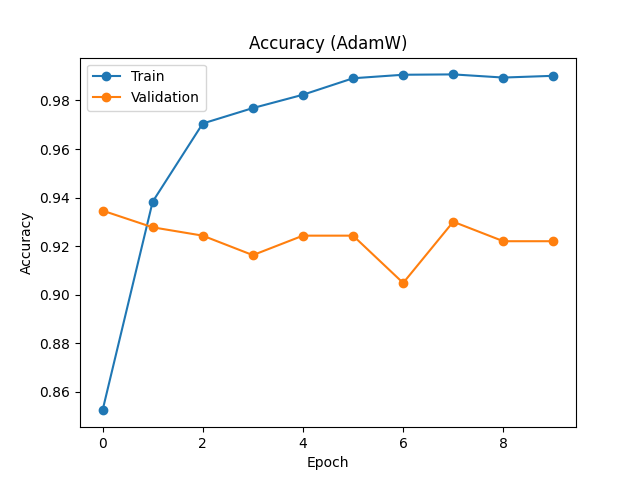
\includegraphics[width=0.3\textwidth]{acc_curve_epoch_10_AdamW.png}
        \caption{AdamW acc curve}\label{AdamW-acc}}%
        \centering
        \parbox[b]{.3\textwidth}{
        \centering
        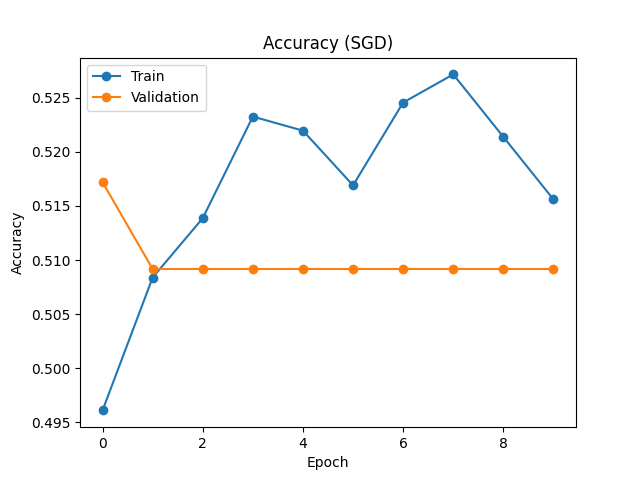
\includegraphics[width=0.3\textwidth]{acc_curve_epoch_10_SGD.png}
        \caption{SGD acc curve}\label{SGD-acc}}
      \end{subcaptiongroup}
    \end{figure}

    \begin{solution}
      I chose SGD and Adagrad to compare with AdamW. SGD is traditional stochastic gradient descent without momentum or weight decay (at least not in my experiment). AdamW is a momentum-based technique with decoupled weight-decay that regularized the weights. Usually, momentum based technique can have faster convergence and better stability which can be shown by comparing SGD and AdamW's plots. We observe that SGD is still unstable at the end of training. In addition, momentum-based methods usually need smaller learning rate while non-momentum-based needs higher learning rate. For the purpose of comparing optimizers, I used the same learning rate $5e-5$ for all runs. We observe that SGD cannot get to good performance and only has around 50\% accuracy. 

      Adagrad is inspired from online learning and the idea of regret. It finds the weird geometry in the previous seen data with the hope to generalize better. Unlike AdamW, Adagrad is not momentum based. We do observe that Adagrad led to a slightly more generalized model in that the validation accuracy is slightly higher than AdamW at the end of training and the validation loss doesn't increase that much compared to AdamW's validation loss.
    \end{solution}
    
    \item[\textbf{Q4.6:}] Experiment with different combinations of \texttt{batch\_size}, \texttt{learning\_rate}, and \texttt{num\_epochs}. Your goal is to pick the final, best model checkpoint based on the validation dataset accuracy. Describe the strategy you used to try different combinations of hyperparameters. Why did you use this strategy?
    
    \begin{solution}
      I did a grid search over 
      \begin{verbatim}
        hyperparams = {
            "batch_size": [64, 128, 256],
            "lr": [1e-4, 5e-5, 1e-5],
            "num_epochs": [2, 5]
        }
      \end{verbatim}

      From previous runs, it seems like there is no need for more epochs because the model just overfits. In addition, all these hyperparameters are run with Adagrad optimizer as a result of observations from previous experiment. I use grid search instead of random search because the search space is small and both \texttt{batch\_size} and \texttt{num\_epochs} are not continuous. Discrete grid search makes sense with learning rate crossing almost one order of magnitude because the default learning rate already works decent in previous run for Adagrad.
    \end{solution}
    
    \item[\textbf{Q4.7:}] What are the \texttt{batch\_size}, \texttt{learning\_rate}, and \texttt{num\_epochs} of the best model checkpoint that you picked? What are the training accuracy and validation accuracy?
    
    \begin{solution}
      The best model is when \texttt{lr=5e-05, batch\_size=128, num\_epochs=5}. The best training and validation accuracy respectively are 95.91\%, 93.23\%.
    \end{solution}
  \end{itemize}
  
  \item[\textit{Step 5:}] \textit{Testing the Final Model}
  \begin{itemize}
      \item[\textbf{Q5.1:}] What's the test set accuracy of the best model?
      
      \begin{solution}
        Test accuracy of best model is 94.83\%
      \end{solution}
  \end{itemize}
    
\end{itemize}

\end{document}